\documentclass[lualatex,handout]{beamer}
\setbeamertemplate{footline}[frame number]
%\useoutertheme{infolines}
\usepackage{luatexja}
\usepackage{xspace}
\usepackage{amsmath,amssymb}
\usepackage{mathtools}

\usepackage{tikz}
\usepackage{pgfplots}
\pgfplotsset{compat=1.18}
\usepackage{gnuplot-lua-tikz}

%\usepackage[haranoaji]{luatexja-preset}
\usepackage[deluxe,ipaex]{luatexja-preset}
\renewcommand{\kanjifamilydefault}{\gtdefault}
%\setmainjfont{HaranoAjiGothic-Regular}

\usepackage{unicode-math}
%\setmathfont{Fira Math}
\setmathfont{STIX Two Math}
\setmathrm{STIX Two Math}[StylisticSet=8]
%\setmathfont{STIX Two Math}[range={up,it,bb,bbit,scr,bfscr},StylisticSet=8]
%\setmathfont{XITS Math}
%\setmathrm{XITS Math}[StylisticSet=8]
%\setmathfont{XITS Math}[StylisticSet=8]

%\usefonttheme{professionalfonts}

\usepackage{luacolor}

%\newcommand{\emm}[1]{\textcolor{red}{#1}}
%\newcommand{\emm}[1]{\color{red}#1\color{black}}
\newcommand{\mycolor}[2]{%
  \begingroup
  \colorlet{currentcolor}{.}%
  \color{#1}#2%
  \color{currentcolor}%
  \endgroup
}
\newcommand{\emm}[1]{\mycolor{red}{#1}}
\newcommand{\expt}[1]{\mathbb{E}\left[#1\right]}
\newcommand{\var}[1]{\mathbb{V}\left[#1\right]}
\newcommand{\cov}[1]{\mathrm{Cov}\left[#1\right]}


\newcommand\bm[1]{{\mathbf{#1}}}
\newcommand\dx{{\,\mathrm{d}x}}


\theoremstyle{definition}

\title{確率・統計基礎: 期待値、分散、モーメント}
\author{森 立平}
\date{}



\begin{document}
\begin{frame}[plain]
\maketitle
\end{frame}

\begin{frame}{確率空間と確率変数}
確率空間$(\Omega,\, P)$
\begin{itemize}
\item $\Omega\colon$ (\emm{非可算}でもよい)集合(\emm{標本空間})
\item $P\colon 2^\Omega\to[0,1]$ (\emm{確率測度})
\end{itemize}
\vspace{1em}
確率の公理
\begin{enumerate}
\setlength{\itemsep}{1em}
\item $P(\Omega)=1$.
\item $\forall (A_n\subseteq\Omega)_{n=1,\dotsc}$, $\forall i\ne j,\, A_i\cap A_j=\emptyset\implies P\left(\bigcup_{n=1}^\infty A_n\right)=\sum_{n=1}^\infty P(A_n)$\\ (\emm{完全加法性, $\sigma$-加法性}).
\end{enumerate}
\vspace{2em}
確率変数(確率空間$(\Omega,\, P)$に付随する)

$X\colon \Omega\to\mathbb{R}$.

\begin{align*}
\Pr(X\in A) &:= P(X^{-1}(A))\qquad \forall A\subseteq\mathbb{R}
\end{align*}
\end{frame}

\begin{frame}{確率変数から定まる確率空間}
\begin{example}
\begin{itemize}
\item $\Omega = \{\mathrm{H},\mathrm{T}\}^2 = \{\mathrm{HH},\mathrm{HT},\mathrm{TH},\mathrm{TT}\}$.
%\item $\mathcal{F} = 2^\Omega$.
\item $P(\{\mathrm{HH}\})=P(\{\mathrm{HT}\})=P(\{\mathrm{TH}\})=P(\{\mathrm{TT}\})=1/4$.
\item $X(\mathrm{HH})=2$, $X(\mathrm{HT})=X(\mathrm{TH})=1$, $X(\mathrm{TT})=0$.
\end{itemize}

このとき、
\begin{align*}
\Pr(X = 0) &= P(\{\mathrm{TT}\}) = 1/4\\
\Pr(X = 1) &= P(\{\mathrm{HT,\,TH}\}) = 1/2\\
\Pr(X = 2) &= P(\{\mathrm{HH}\}) = 1/4
\end{align*}
である
\end{example}
\begin{center}
そもそも最初から確率空間
\begin{itemize}
\item $\Omega = \{0,1,2\}$.
\item $P(\{0\}) = 1/4, P(\{1\}) = 1/2, P(\{2\}) = 1/4$
\end{itemize}

を考えればよいのでは?
%一般に$(\mathbb{R},\, Q(A) := P(X \in A))$
\end{center}
\end{frame}

\begin{frame}{複数の確率変数}
\begin{example}
\begin{itemize}
\item $\Omega = \{\mathrm{H},\mathrm{T}\}^2 = \{\mathrm{HH},\mathrm{HT},\mathrm{TH},\mathrm{TT}\}$.
%\item $\mathcal{F} = 2^\Omega$.
\item $P(\{\mathrm{HH}\})=P(\{\mathrm{HT}\})=P(\{\mathrm{TH}\})=P(\{\mathrm{TT}\})=1/4$.
\item $X(\mathrm{HH})=2$, $X(\mathrm{HT})=X(\mathrm{TH})=1$, $X(\mathrm{TT})=0$.
\item $Y(\mathrm{HH})=Y(\mathrm{HT})=1$, $Y(\mathrm{TH})=Y(\mathrm{TT})=0$.
\end{itemize}

このとき、
\begin{align*}
\Pr(X = 0,\, Y = 0) &= P(X^{-1}(0)\cap Y^{-1}(0)) = P(\{\mathrm{TT}\}) = 1/4\\
\Pr(X = 0,\, Y = 1) &= P(X^{-1}(0)\cap Y^{-1}(1)) =P(\emptyset) = 0\\
\Pr(X = 1,\, Y = 0) &= P(X^{-1}(1)\cap Y^{-1}(0)) =P(\{\mathrm{TH}\}) = 1/4\\
\Pr(X = 1,\, Y = 1) &= P(X^{-1}(1)\cap Y^{-1}(1)) =P(\{\mathrm{HT}\}) = 1/4\\
\Pr(X = 2,\, Y = 0) &= P(X^{-1}(2)\cap Y^{-1}(0)) =P(\emptyset) = 0\\
\Pr(X = 2,\, Y = 1) &= P(X^{-1}(2)\cap Y^{-1}(1)) =P(\{\mathrm{HH}\}) = 1/4
\end{align*}
である。複数の確率変数を考えるときには確率空間は必要。
\end{example}
\end{frame}

\begin{frame}{連続確率空間}
$\Omega = \mathbb{R}$の場合の確率空間$(\mathbb{R},\, P)$について考える。

\vspace{1em}
ある積分できる関数$p\colon\mathbb{R}\to\mathbb{R}$が存在して
\begin{align*}
P([a,b]) &= \int_a^{b} p(x)\dx
\end{align*}
であるとき、$p$を\emm{確率密度関数}という。

\vspace{1em}
確率密度関数は常に存在するとは限らないが累積分布関数$F_X(a) = \Pr(X\le a)$は常に存在する。
\end{frame}

\begin{frame}{一様分布}
\begin{align*}
\Omega &= [0,\, 1]\\
p(x) &= 1,& \Pr(X\le x) = x
\end{align*}
\begin{tikzpicture}
\begin{axis}[
    width=0.45\textwidth,
    xlabel=$x$,
    ylabel=$p(x)$,
    xmin=0, xmax=1,
    ymin=0, ymax=1.2,
    xtick={0,0.5,1},
    ytick={0,0.5,1}
]
    \addplot[domain=0:1, samples=100, color=blue, thick] {1};
\end{axis}
\end{tikzpicture}
\hfill
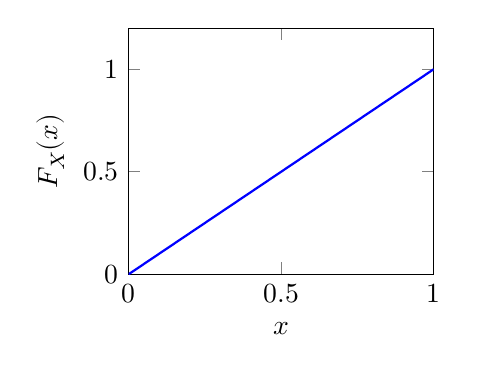
\begin{tikzpicture}
\begin{axis}[
    width=0.45\textwidth,
    xlabel=$x$,
    ylabel=$F_X(x)$,
    xmin=0, xmax=1,
    ymin=0, ymax=1.2,
    xtick={0,0.5,1},
    ytick={0,0.5,1}
]
    \addplot[domain=0:1, samples=100, color=blue, thick] {x};
\end{axis}
\end{tikzpicture}
\end{frame}

\begin{frame}{標準正規分布(標準ガウス分布)}
\begin{align*}
\Omega &= \mathbb{R}\\
p(x) &= \frac1{\sqrt{2\pi}} \mathrm{e}^{-\frac{x^2}{2}},& \Pr(X\le x) = \Phi(x) := \frac1{\sqrt{2\pi}}\int_{-\infty}^x \mathrm{e}^{-\frac{t^2}2} \,\mathrm{d}t
\end{align*}
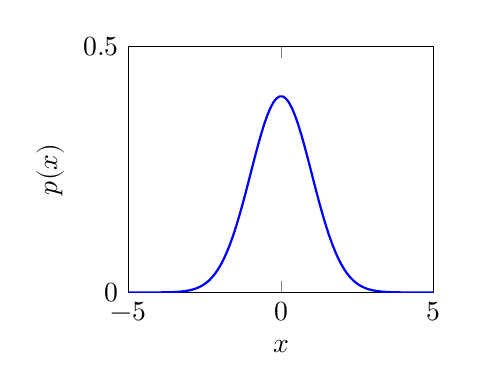
\begin{tikzpicture}
\begin{axis}[
    width=0.45\textwidth,
    xlabel=$x$,
    ylabel=$p(x)$,
    xmin=-5, xmax=5,
    ymin=0, ymax=0.5,
    xtick={-5,0,5},
    ytick={0,0.5,1}
]
    \addplot[domain=-5:5, samples=100, color=blue, thick] {exp(-x^2/2)/sqrt(2*pi)};
\end{axis}
\end{tikzpicture}
\hfill
\begin{tikzpicture}
\begin{axis}[
    width=0.45\textwidth,
    xlabel=$x$,
    ylabel=$F_X(x)$,
    xmin=-5, xmax=5,
    ymin=0, ymax=1,
    xtick={-5,0,5},
    ytick={0,0.5,1}
]
    %%\addplot[domain=-5:5, samples=100, color=blue, thick] {0.5*(1 + erf(x/sqrt(2)))};
 \addplot[samples=100, color=blue, no markers, thick] gnuplot {0.5*(1 + erf(x/sqrt(2)))};
\end{axis}
\end{tikzpicture}
\end{frame}

\begin{frame}{指数分布}
\begin{align*}
\Omega &= [0,\, \infty)\\
p(x) &= \lambda\mathrm{e}^{-\lambda x},& \Pr(X\le x) = 1-\mathrm{e}^{-\lambda x}
\end{align*}
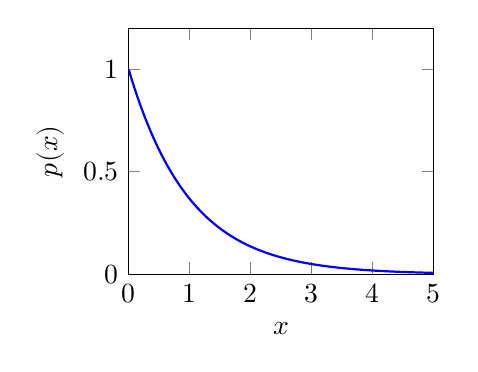
\begin{tikzpicture}
\begin{axis}[
    width=0.45\textwidth,
    xlabel=$x$,
    ylabel=$p(x)$,
    xmin=0, xmax=5,
    ymin=0, ymax=1.2,
    xtick={0,1,2,3,4,5},
    ytick={0,0.5,1}
]
    \addplot[domain=0:5, samples=100, color=blue, thick] {exp(-x)};
\end{axis}
\end{tikzpicture}
\hfill
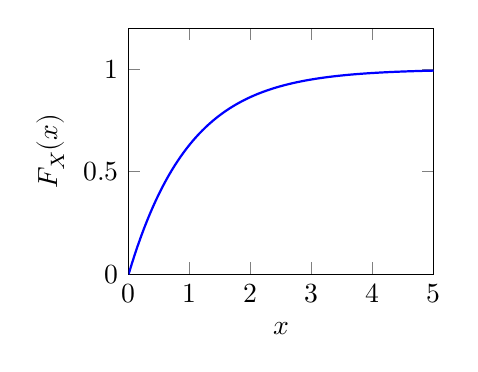
\begin{tikzpicture}
\begin{axis}[
    width=0.45\textwidth,
    xlabel=$x$,
    ylabel=$F_X(x)$,
    xmin=0, xmax=5,
    ymin=0, ymax=1.2,
    xtick={0,1,2,3,4,5},
    ytick={0,0.5,1}
]
    \addplot[domain=0:5, samples=100, color=blue, thick] {1-exp(-x)};
\end{axis}
\end{tikzpicture}
\end{frame}

\begin{frame}{標準コーシー分布}
\begin{align*}
\Omega &= \mathbb{R}\\
p(x) &= \frac1{\pi(1+x^2)},& \Pr(X\le x) = \frac1\pi\arctan(x) + \frac12
\end{align*}
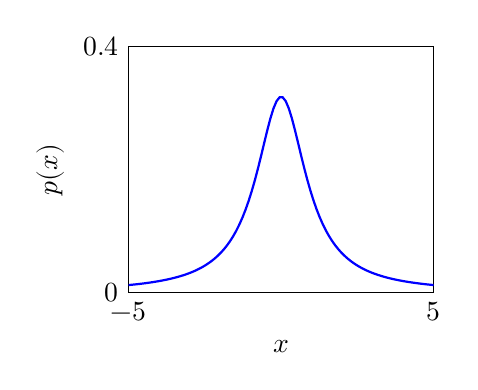
\begin{tikzpicture}
\begin{axis}[
    width=0.45\textwidth,
    xlabel=$x$,
    ylabel=$p(x)$,
    xmin=-5, xmax=5,
    ymin=0, ymax=0.4,
    xtick={-5,5},
    ytick={0,0.4}
]
    \addplot[domain=-5:5, samples=100, color=blue, thick] {1/(pi*(1+x^2)};
\end{axis}
\end{tikzpicture}
\hfill
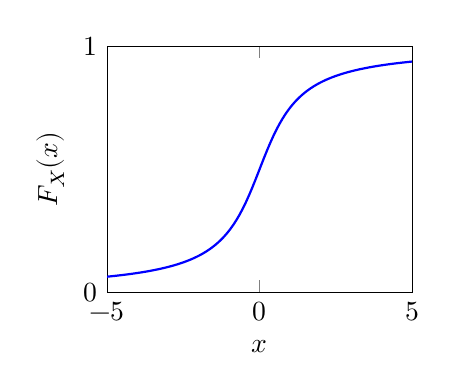
\begin{tikzpicture}
\begin{axis}[
    width=0.45\textwidth,
    xlabel=$x$,
    ylabel=$F_X(x)$,
    xmin=-5, xmax=5,
    ymin=0, ymax=1,
    xtick={-5,0,5},
    ytick={0,1}
]
    \addplot[domain=-5:5, samples=100, color=blue, thick] {atan(x)/180 + 0.5};
\end{axis}
\end{tikzpicture}
\end{frame}

\begin{frame}{期待値(平均)}
非負離散確率変数$X$について
\begin{align*}
\expt{X} &:= \sum_k \Pr(X=k) k\qquad\text{(収束するとき)}
\end{align*}

\vspace{1em}
離散確率変数$X$について$\expt{|X|}=\sum_k \Pr(X=k)|k|$が存在するとき、
\begin{align*}
\expt{X} &:= \sum_k \Pr(X=k) k
\end{align*}

\vspace{1em}
連続確率変数$X$について
\begin{align*}
\expt{X} &:= \int p(x) x \dx
\end{align*}
\end{frame}

\begin{frame}{期待値の線形性}
\small
\begin{align*}
\expt{f(X)} &= \sum_k \Pr(f(X) = k) k\\
&= \sum_k \Pr(X \in f^{-1}(k)) k\\
&= \sum_k \sum_{t\in f^{-1}(k)} \Pr(X = t) k\\
&= \sum_t \Pr(X = t) f(t)
\end{align*}
\begin{align*}
\expt{aX + bY} &= \sum_k \Pr(aX+bY=k) k\\
&= \sum_{x, y} \Pr(X=x, Y=y) (ax+by)\\
&= \sum_{x, y} \Pr(X=x, Y=y) ax + \sum_{x, y} \Pr(X=x, Y=y) by\\
&= \sum_{x} \Pr(X=x) ax + \sum_{y} \Pr(Y=y) by\\
&= a\sum_{x} \Pr(X=x) x + b\sum_{y} \Pr(Y=y) y\\
&=a\expt{X} + b\expt{Y} 
\end{align*}
\end{frame}

\begin{frame}{積の期待値}
\emm{独立な}確率変数$X$と$Y$について
\begin{align*}
\expt{XY} &= \sum_{k} \Pr(XY = k)\, k\\
&= \sum_{x,y}\Pr(X=x,Y=y)\, xy\\
&= \sum_{x,y}\Pr(X=x)\Pr(Y=y)\, xy\\
&= \left(\sum_{x}\Pr(X=x)\right)\left(\sum_y \Pr(Y=y)y\right)\\
&= \expt{X}\expt{Y}
\end{align*}
\end{frame}

\begin{frame}{期待値の例}
\begin{example}[ベルヌーイ分布]
\begin{align*}
\Pr(X = 0) &= 1-p\\
\Pr(X = 1) &= p\\
\end{align*}
のとき、
\begin{align*}
\expt{X} &= \Pr(X = 0)\cdot 0 + \Pr(X = 1)\cdot 1\\
&= p
\end{align*}
\end{example}

\end{frame}

\begin{frame}{期待値の例}
\begin{example}[二項分布]
\begin{align*}
\Pr(X = k) &= \binom{n}{k} p^k(1-p)^{n-k}
\end{align*}
のとき、
\begin{align*}
\expt{X} &= \sum_k \Pr(X = k) k\\
&= \binom{n}{k} p^k(1-p)^{n-k} k
\end{align*}
一方で$t$回目のコイン投げで表が出たら1、裏が出たら0という確率変数を$X_t$とおくと、
$X=X_1+X_2+\dotsb+X_n$なので
\begin{align*}
\expt{X} &= \expt{X_1+\dotsb+X_n} = \expt{X_1}+\dotsb+\expt{X_n} = np.
\end{align*}
\end{example}
\end{frame}

\begin{frame}{期待値の例}
\begin{example}[標準正規分布]
\begin{align*}
p(x) &= \frac1{\sqrt{2\pi}} \mathrm{e}^{-\frac{x^2}{2}}
\end{align*}
のとき、
\begin{align*}
\expt{X} &= \int_{-\infty}^{\infty} p(x) x\dx\\
&= \int_{-\infty}^\infty \frac1{\sqrt{2\pi}} \mathrm{e}^{-\frac{x^2}{2}} x\dx\\
&=\left[-\frac1{\sqrt{2\pi}} \mathrm{e}^{-\frac{x^2}2}\right]_{-\infty}^\infty = 0
\end{align*}
\end{example}
\end{frame}

\begin{frame}{期待値の例}
\begin{example}[正規分布]
\begin{align*}
p(x) &= \frac1{\sqrt{2\pi}} \mathrm{e}^{-\frac{(x-\emm{m})^2}{2}}
\end{align*}
のとき、
\begin{align*}
\expt{X} &= \int_{-\infty}^{\infty} p(x) x\dx\\
&= \int_{-\infty}^\infty \frac1{\sqrt{2\pi}} \mathrm{e}^{-\frac{(x-\emm{m})^2}{2}} x\dx\\
&= \int_{-\infty}^\infty \frac1{\sqrt{2\pi}} \mathrm{e}^{-\frac{x^2}{2}} (x+\emm{m})\dx\\
&= \int_{-\infty}^\infty \frac1{\sqrt{2\pi}} \mathrm{e}^{-\frac{x^2}{2}} \emm{m}\dx = \emm{m}
\end{align*}
\end{example}
\end{frame}

\begin{frame}{期待値の例}
\begin{example}[コーシー分布]
\begin{align*}
p(x) &= \frac1{\pi(1+x^2)}
\end{align*}
のとき、
\begin{align*}
\expt{X} &= \int_{-\infty}^{\infty} p(x) x\dx\\
&= \int_{-\infty}^\infty \frac1{\pi(1+x^2)} x\dx\\
&= \frac1{2\pi} \int_{-\infty}^\infty \left(\frac{1}{x+i} + \frac{1}{x-i}\right)\dx\\
\end{align*}
\end{example}
\end{frame}

\begin{frame}{マルコフの不等式}
\begin{theorem}[マルコフの不等式]
任意の\emm{非負}の確率変数$X$と$a>0$について
\begin{align*}
\Pr(X\ge a) &\le \frac{\expt{X}}{a}
\end{align*}
\end{theorem}
\begin{proof}
\vspace{-2em}
\begin{align*}
\expt{X} &= \sum_k \Pr(X=k)k\\
&= \sum_{k \ge a} \Pr(X=k)k
+ \sum_{k < a} \Pr(X=k)k\\
&\ge \sum_{k \ge a} \Pr(X=k)k\hspace{8em}(k\ge 0)\\
&\ge \sum_{k \ge a} \Pr(X=k)a\\
&= a\Pr(X\ge a). \qedhere
\end{align*}
\end{proof}
\end{frame}

%\begin{frame}{例題}
%\end{frame}

\begin{frame}{分散}
\begin{align*}
\var{X} &:= \expt{(X-\expt{X})^2}\\
&=\expt{X^2-2X\expt{X}+\expt{X}^2}\\
&=\expt{X^2}-2\expt{X}\expt{X}+\expt{X}^2\\
&=\emm{\expt{X^2}-\expt{X}^2}\\
\end{align*}
\begin{center}
分散は\emm{非負}で\emm{期待値からの広がり}を表す量。
\end{center}

\vspace{1em}
$\var{X} = 0 \iff \Pr(X = \expt{X})=1$.
\end{frame}

%\begin{frame}{分散の意味}
%\begin{align*}
%\var{X} &= \expt{(X-\expt{X})^2}
%\end{align*}
%
%\end{frame}

\begin{frame}{分散の性質}
\small
\begin{align*}
\var{X} &= \expt{(X-\expt{X})^2}
\end{align*}
%\vspace{1em}
\begin{align*}
\var{aX} &= \expt{(aX-\expt{aX})^2}\\
&= \expt{(aX-a\expt{X})^2}\\
&= \expt{a^2(X-\expt{X})^2}\\
&= a^2\expt{(X-\expt{X})^2}\\
&= a^2\var{X}
\end{align*}
%
\begin{align*}
\var{X+Y} &= \expt{(X+Y-\expt{X+Y})^2}\\
 &= \expt{(X-\expt{X}+Y-\expt{Y})^2}\\
 &= \expt{(X-\expt{X})^2+(Y-\expt{Y})^2 + 2(X-\expt{X})(Y-\expt{Y})}\\
 &= \expt{(X-\expt{X})^2}+\expt{(Y-\expt{Y})^2} + 2\expt{(X-\expt{X})(Y-\expt{Y})}\\
 &= \var{X}+\var{Y}+ 2\emm{\expt{(X-\expt{X})(Y-\expt{Y})}}\\
\end{align*}
\end{frame}

\begin{frame}{共分散}
\begin{align*}
\cov{X,Y} &:= \expt{(X-\expt{X})(Y-\expt{Y})}
\end{align*}

\vspace{1em}

\begin{itemize}
\setlength{\itemsep}{2em}
\item $X-\expt{X}$と$Y-\expt{Y}$の符号が一緒 $\Rightarrow$ $\cov{X,Y}\ge 0$。
\item $X-\expt{X}$と$Y-\expt{Y}$の符号が逆 $\Rightarrow$ $\cov{X,Y}\le 0$。
\end{itemize}

\vspace{1em}
直感的な意味

\vspace{1em}
\begin{itemize}
\setlength{\itemsep}{2em}
\item $X$が大きいとき$Y$が大きい $\Rightarrow$ $\cov{X,Y}\ge 0$。
\item $X$が大きいとき$Y$が小さい $\Rightarrow$ $\cov{X,Y}\le 0$。
\end{itemize}
\end{frame}

\begin{frame}{無相関と独立}
\begin{align*}
\cov{X,Y} &= \expt{(X-\expt{X})(Y-\expt{Y})}
\end{align*}
\vspace{1em}
確率変数$X$と$Y$が\emm{無相関} $\stackrel{\mathrm{def}}{\iff} \cov{X,Y}=0$

\vspace{1em}
確率変数$X$と$Y$が独立 $\Longrightarrow \cov{X,Y} = \expt{(X-\expt{X})(Y-\expt{Y})} = \expt{X-\expt{X}}\expt{Y-\expt{Y}} = 0\iff$
確率変数$X$と$Y$が\emm{無相関}

\vspace{1em}
無相関だけど独立でない例

\begin{align*}
\Pr(X=1, Y=0) &= \frac12\\
\Pr(X=-1, Y=1) &= \frac14\\
\Pr(X=-1, Y=-1) &= \frac14
\end{align*}
\end{frame}

\begin{frame}{チェビシェフの不等式}
\begin{lemma}[チェビシェフの不等式]
確率変数$X$が分散を持つと仮定する。任意の $a>0$について
\begin{align*}
\Pr(|X-\expt{X}|\ge a) &\le \frac{\var{X}}{a^2}
\end{align*}
\end{lemma}
\begin{proof}
\begin{align*}
\Pr(|X-\expt{X}|\ge a) &=\Pr((X-\expt{X})^2\ge a^2)\\
&\le\frac{\expt{(X-\expt{X})^2}}{a^2}\hspace{3em}\text{(マルコフの不等式)}
\end{align*}
\end{proof}
\end{frame}

\begin{frame}{モーメント母関数}
確率変数$X$の\emm{$n$次モーメント}: $\expt{X^n}$.

\vspace{1em}
確率変数$X$の\emm{モーメント母関数(積率母関数)}: $M_X(t):=\expt{\mathrm{e}^{tX}}$.

モーメント母関数が\emm{$t\in(-\epsilon,\epsilon)$で存在}するとき、この範囲で
\begin{align*}
M_X(t)&=\expt{\mathrm{e}^{tX}}\\
&= \expt{\sum_{n\ge 0} \frac{(tX)^n}{n!}}\\
&= \sum_{n\ge 0} \expt{\frac{(tX)^n}{n!}}\qquad(\text{極限と積分の交換})\\
&= \sum_{n\ge 0} \frac{\expt{X^n}}{n!} t^n\\
&= 1 + \expt{X}t + \frac{\expt{X^2}}2t^2 + \dotsb
\end{align*}
\begin{align*}
%\left.\frac{\mathrm{d} M_X(t)}{\mathrm{d}t}\right|_{t=0} &= \expt{X},&
%\left.\frac{\mathrm{d}^2 M_X(t)}{\mathrm{d}t^2}\right|_{t=0} &= \expt{X^2}
\left.\frac{\mathrm{d}^n M_X(t)}{\mathrm{d}t^n}\right|_{t=0} &= \expt{X^n}\qquad n\ge 0
\end{align*}
\end{frame}

\begin{frame}{モーメント母関数の例}
\small
\begin{example}[二項分布]
\begin{align*}
\Pr(X = k) &= \binom{n}{k} p^k(1-p)^{n-k}
\end{align*}
のとき、
\begin{align*}
M_X(t)&=\mathbb{E}[\mathrm{e}^{tX}]\\
&=\sum_k \Pr(X=k)\mathrm{e}^{tk}\\
&=\sum_k \binom{n}{k}p^k(1-p)^{n-k}\mathrm{e}^{tk}\\
&=(p\mathrm{e}^t + (1-p))^n
\end{align*}
\begin{align*}
\left.\frac{\mathrm{d} M_X(t)}{\mathrm{d}t}\right|_{t=0} &= \left.n(p\mathrm{e}^t + (1-p))^{n-1}p\mathrm{e}^t\right|_{t=0}=np
\end{align*}
\end{example}
\end{frame}

\begin{frame}{独立確率変数の和のモーメント母関数}
\emm{独立}確率変数$X$と$Y$について
\begin{align*}
M_{X+Y}(t) &= \expt{\mathrm{e}^{t(X+Y)}}\\
&= \expt{\mathrm{e}^{tX}}\expt{\mathrm{e}^{tY}}\\
&=M_X(t)M_Y(t)
\end{align*}

ベルヌーイ分布のモーメント母関数は
\begin{align*}
M_{X}(t) &= \expt{\mathrm{e}^{tX}}\\
&=p\mathrm{e}^t + (1-p)
\end{align*}

二項分布に従う確率変数はベルヌーイ分布に従う$n$個の独立確率変数の和なので、そのモーメント母関数は
\begin{align*}
(p\mathrm{e}^t + (1-p))^n
\end{align*}
\end{frame}

\begin{frame}{キュムラント母関数}
\emm{キュムラント母関数 $K_X(t)$}は以下で定義される。
\begin{align*}
K_X(t) &:= \log(M_X(t)) = \log\expt{\mathrm{e}^{tX}}
\end{align*}
\begin{align*}
\left.\frac{\mathrm{d} K_X(t)}{\mathrm{d}t}\right|_{t=0} &= \expt{X},&
\left.\frac{\mathrm{d}^2 K_X(t)}{\mathrm{d}t^2}\right|_{t=0} &= \expt{X^2} - \expt{X}^2 = \var{X}
\end{align*}

\vspace{2em}
\emm{独立}確率変数$X$と$Y$について
\begin{align*}
K_{X+Y}(t) &= K_X(t) + K_Y(t).
\end{align*}
\end{frame}

\if0
\begin{frame}{コーシー・シュワルツの不等式}
\begin{theorem}
\begin{align*}
\expt{XY}^2 \le \expt{X^2}\expt{Y^2}
\end{align*}
\end{theorem}
\end{frame}

\begin{frame}{イェンセンの不等式}
\begin{theorem}
凸関数$f\colon\mathbb{R}\to\mathbb{R}$について
\begin{align*}
\expt{f(X)} \ge f(\expt{X})
\end{align*}
\end{theorem}

\end{frame}
\fi

%モーメント母関数、畳み込み
\begin{frame}{課題}
\begin{itemize}
\setlength{\itemsep}{2em}
\item 標準正規分布のモーメント母関数、期待値、分散をもとめよ。
\item $\lambda>0$について、非負整数上の分布であるポアソン分布$\Pr(X=k)=\frac{\lambda^k}{k!}\mathrm{e}^{-\lambda}$のモーメント母関数、期待値、分散をもとめよ。
\item $\lambda>0$について、非負実数上の分布である指数分布$p(x)=\lambda\mathrm{e}^{-\lambda x}$のモーメント母関数、期待値、分散をもとめよ。
モーメント母関数が存在する$t$の範囲も示すこと。
%\item 幾何分布$\Pr(X=k)=(1-p)^{k-1}p$のモーメント母関数、期待値、分散をもとめよ
%\item 
\end{itemize}
\end{frame}

\end{document}
